\documentclass[10pt,a4paper]{article}
\usepackage[utf8]{inputenc}
\usepackage[spanish]{babel}
\usepackage{amsmath}
\usepackage{amsfonts}
\usepackage{amssymb}
\usepackage{makeidx}
\usepackage{graphicx}
\usepackage{fourier}
\usepackage[left=2cm,right=2cm,top=2cm,bottom=2cm]{geometry}
\author{M.Sabogal}
\begin{document}

\section{Solucion para un tiempo t=40 (u.a)}
\begin{figure}[h!]
\centering 
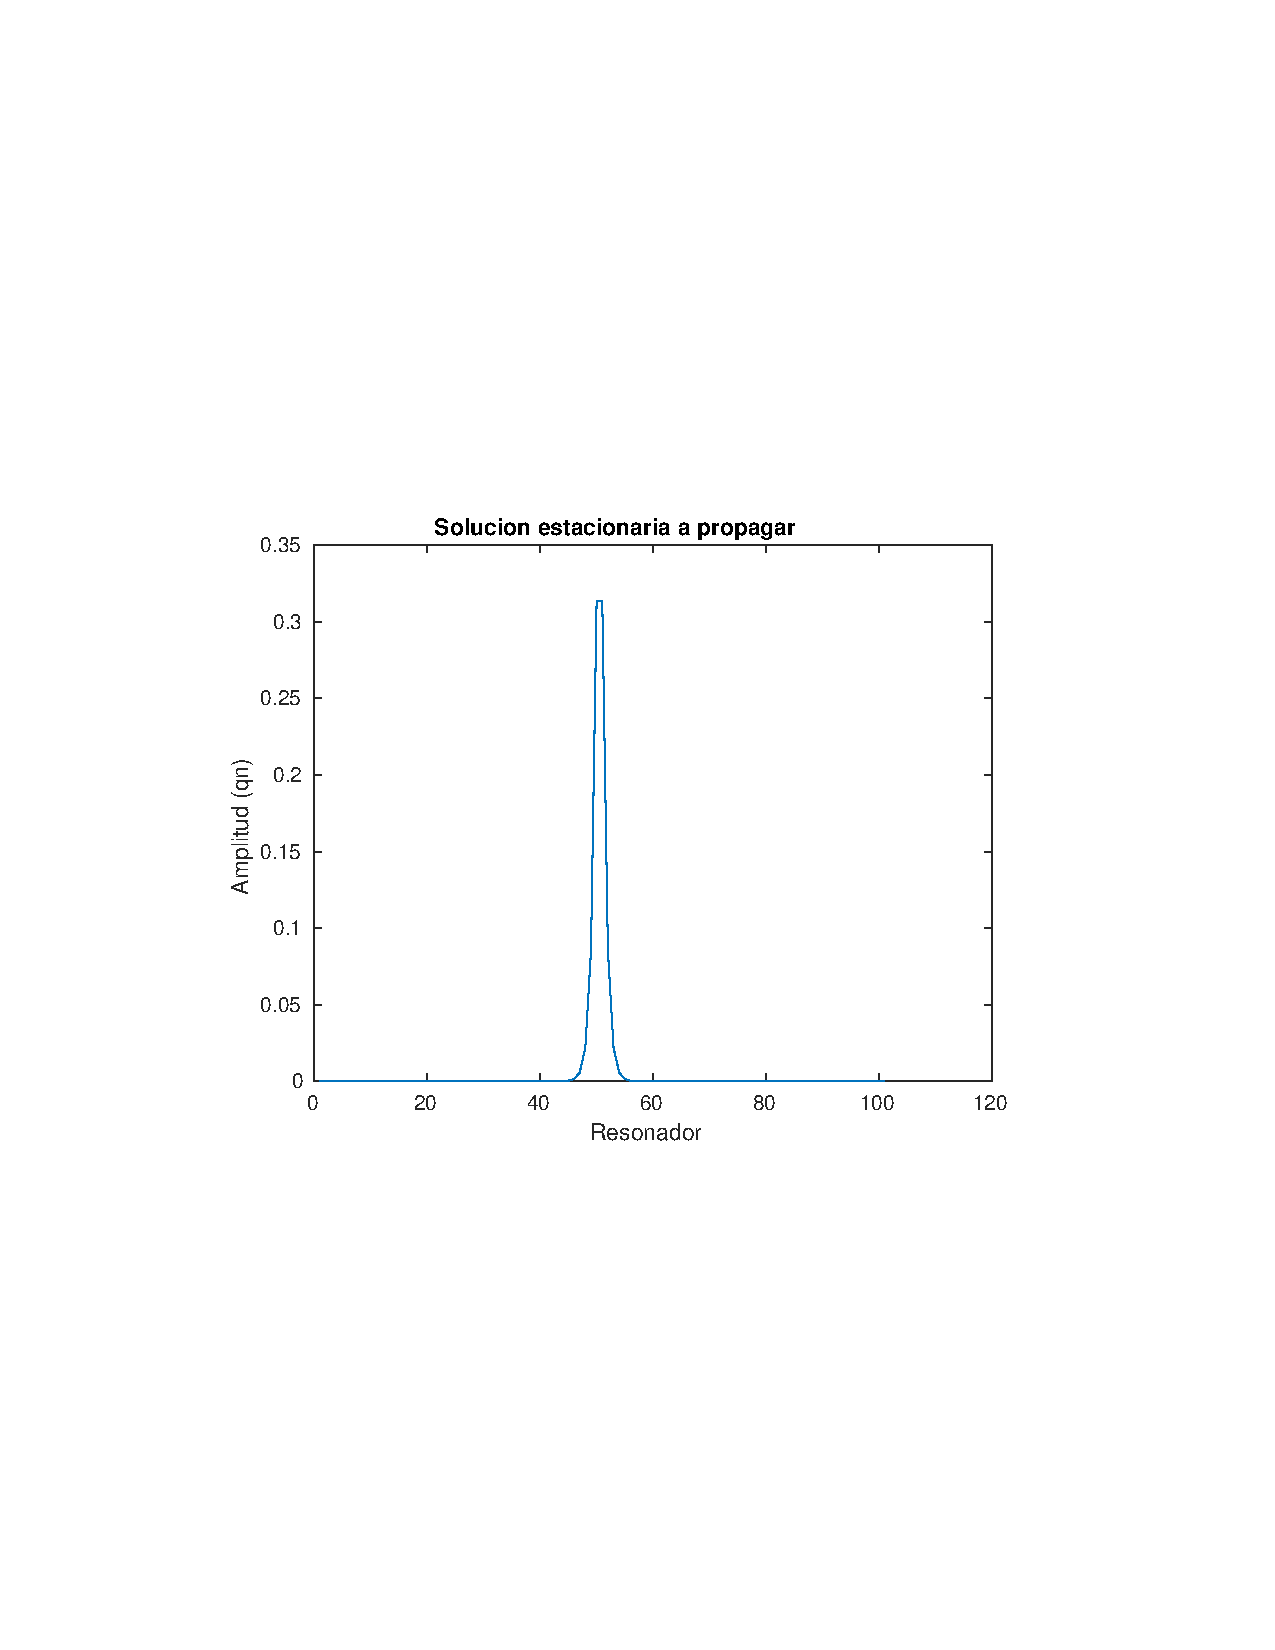
\includegraphics[scale=0.8]{SE2.pdf}
\end{figure}

\begin{figure}[h!]
\centering 
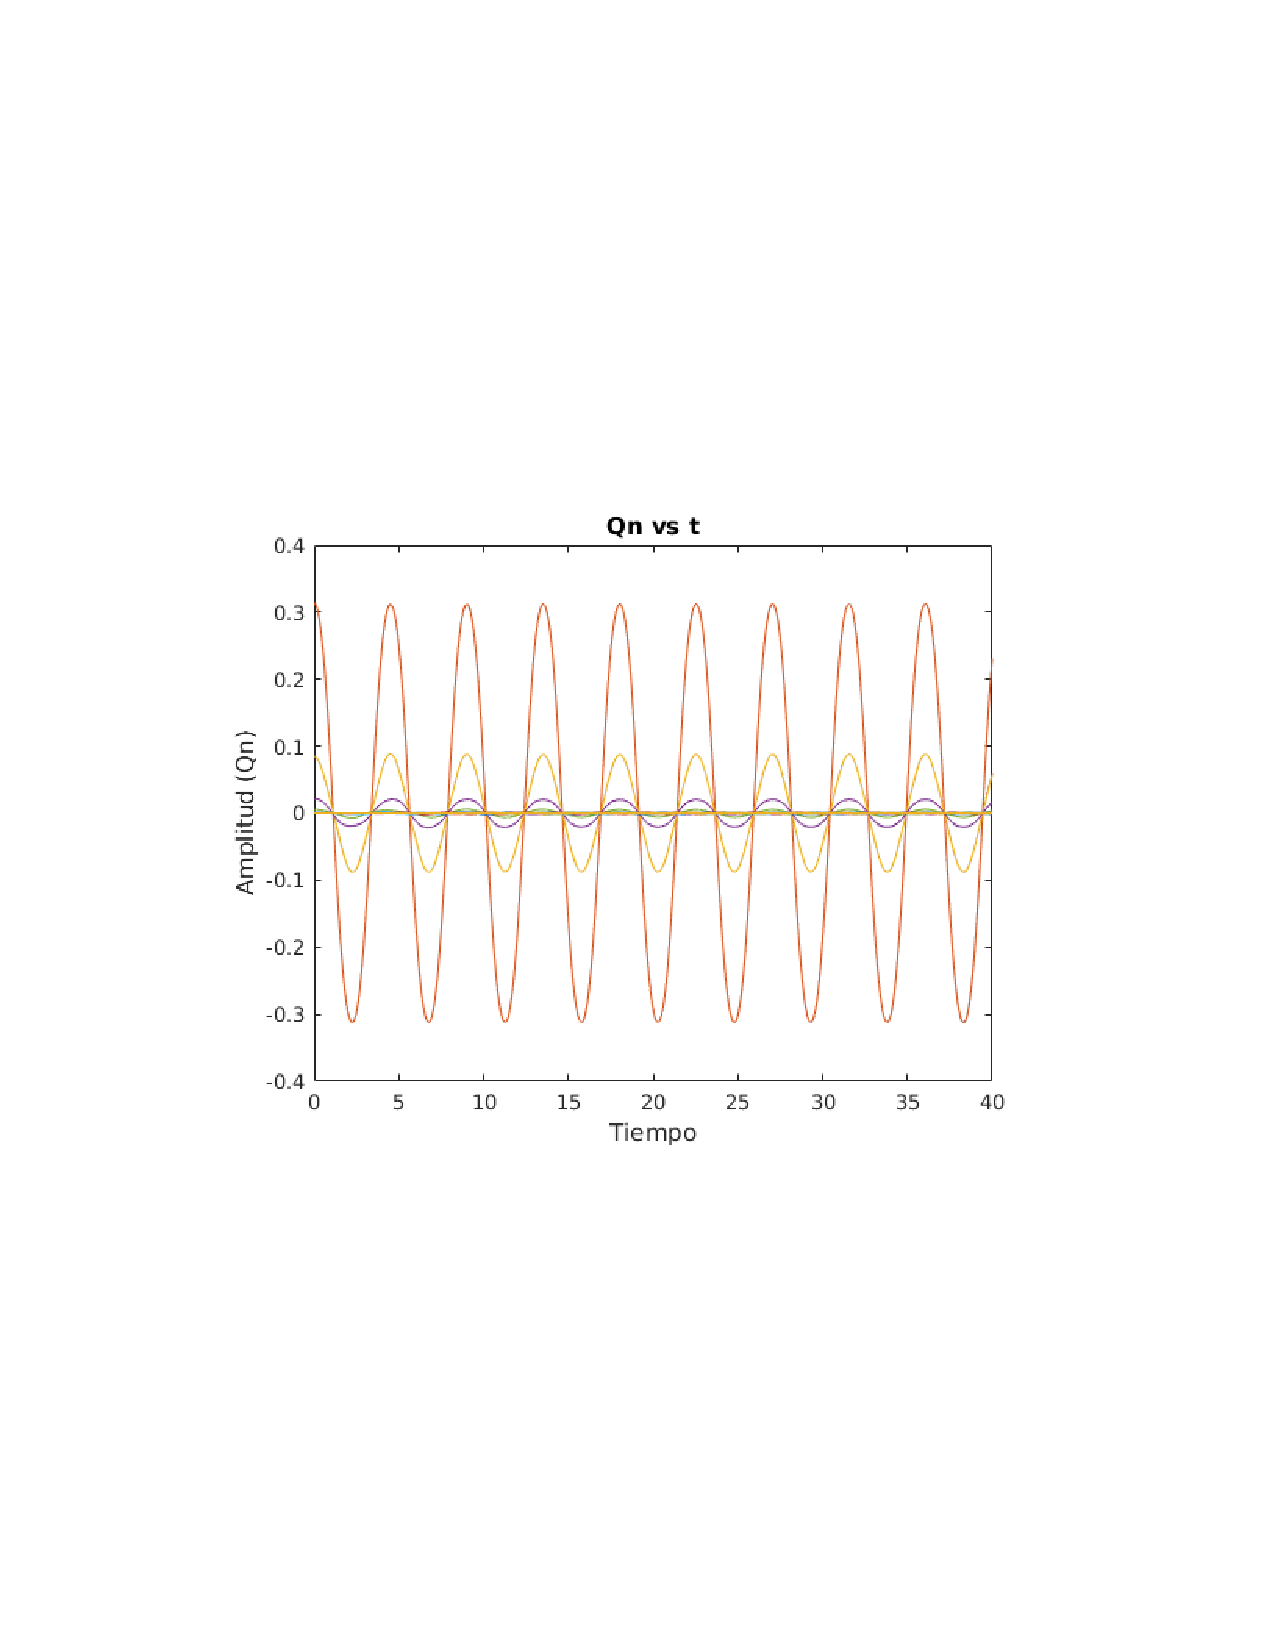
\includegraphics[scale=0.8]{Qn2-40.pdf}
\end{figure}


\begin{figure}[h!]
\centering 
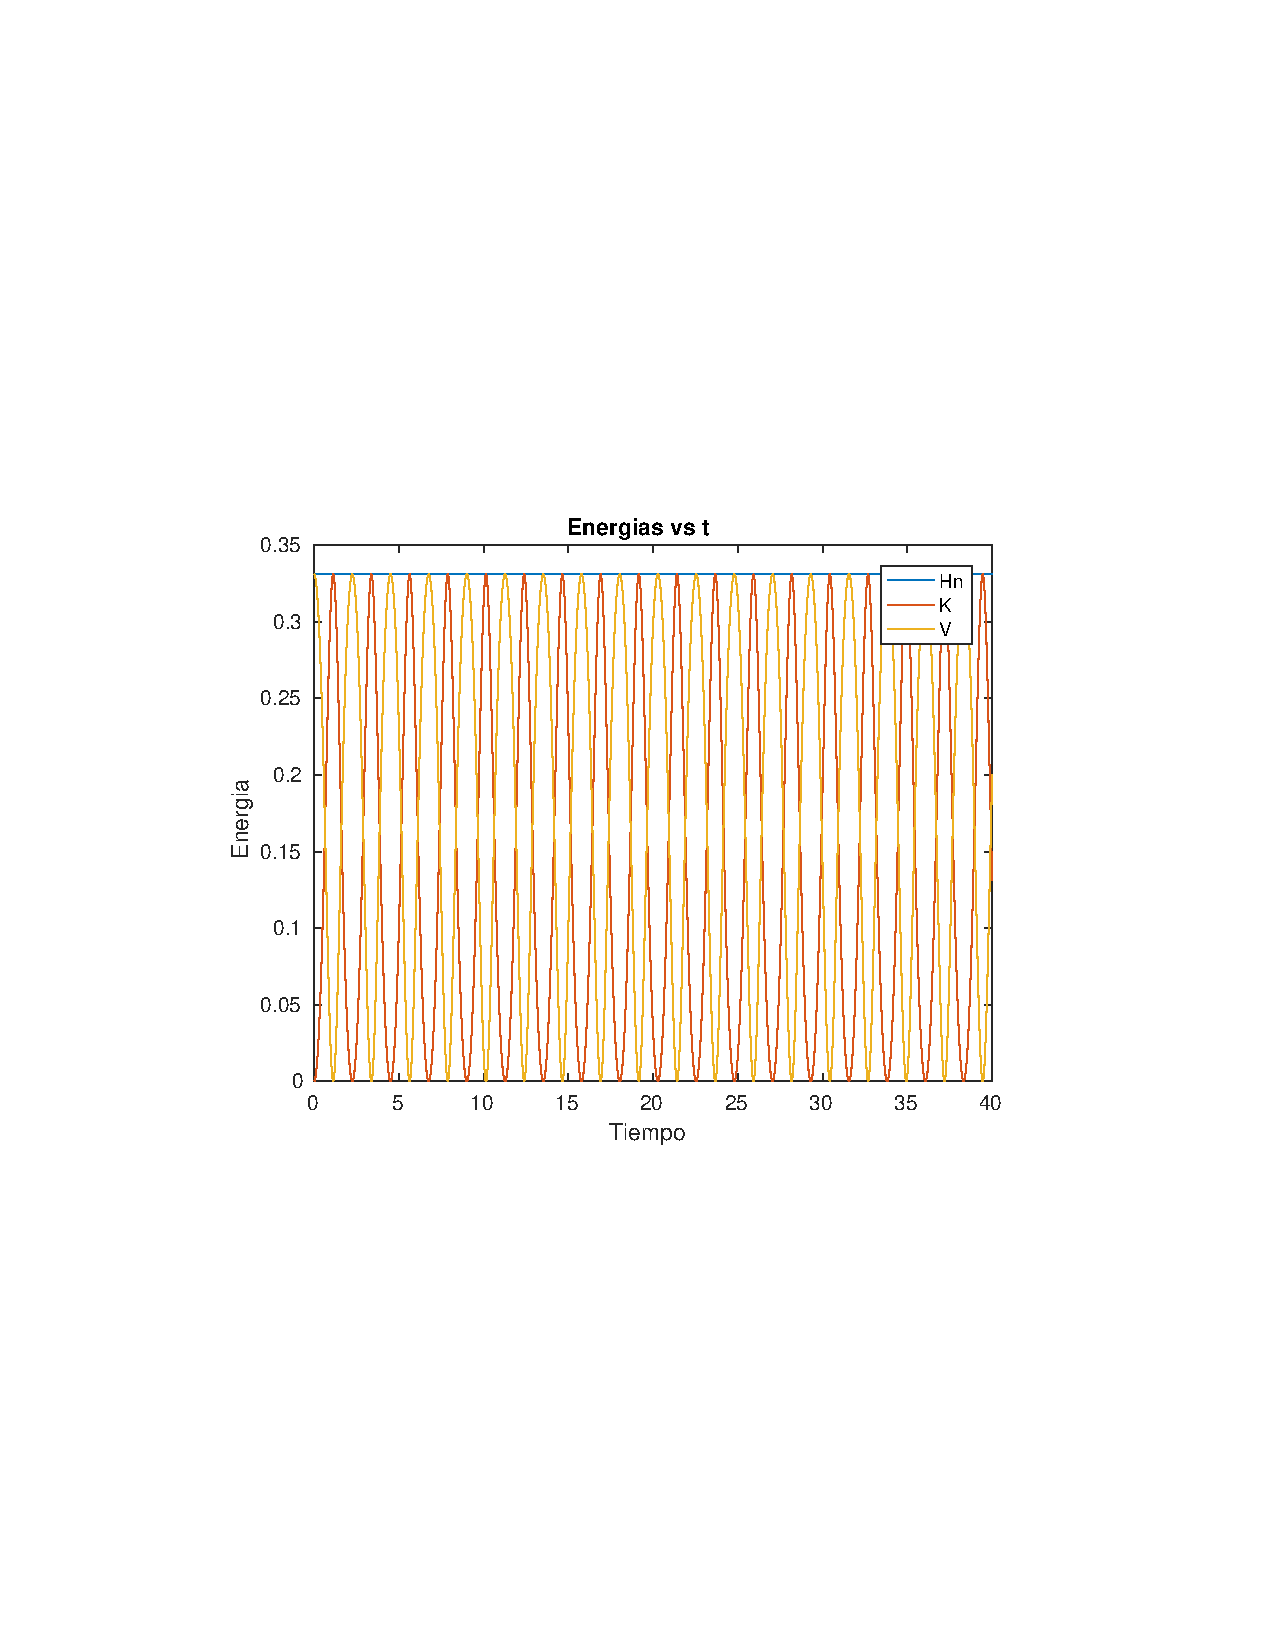
\includegraphics[scale=0.8]{E2-40.pdf}
\end{figure}


\begin{figure}[h!]
\centering 
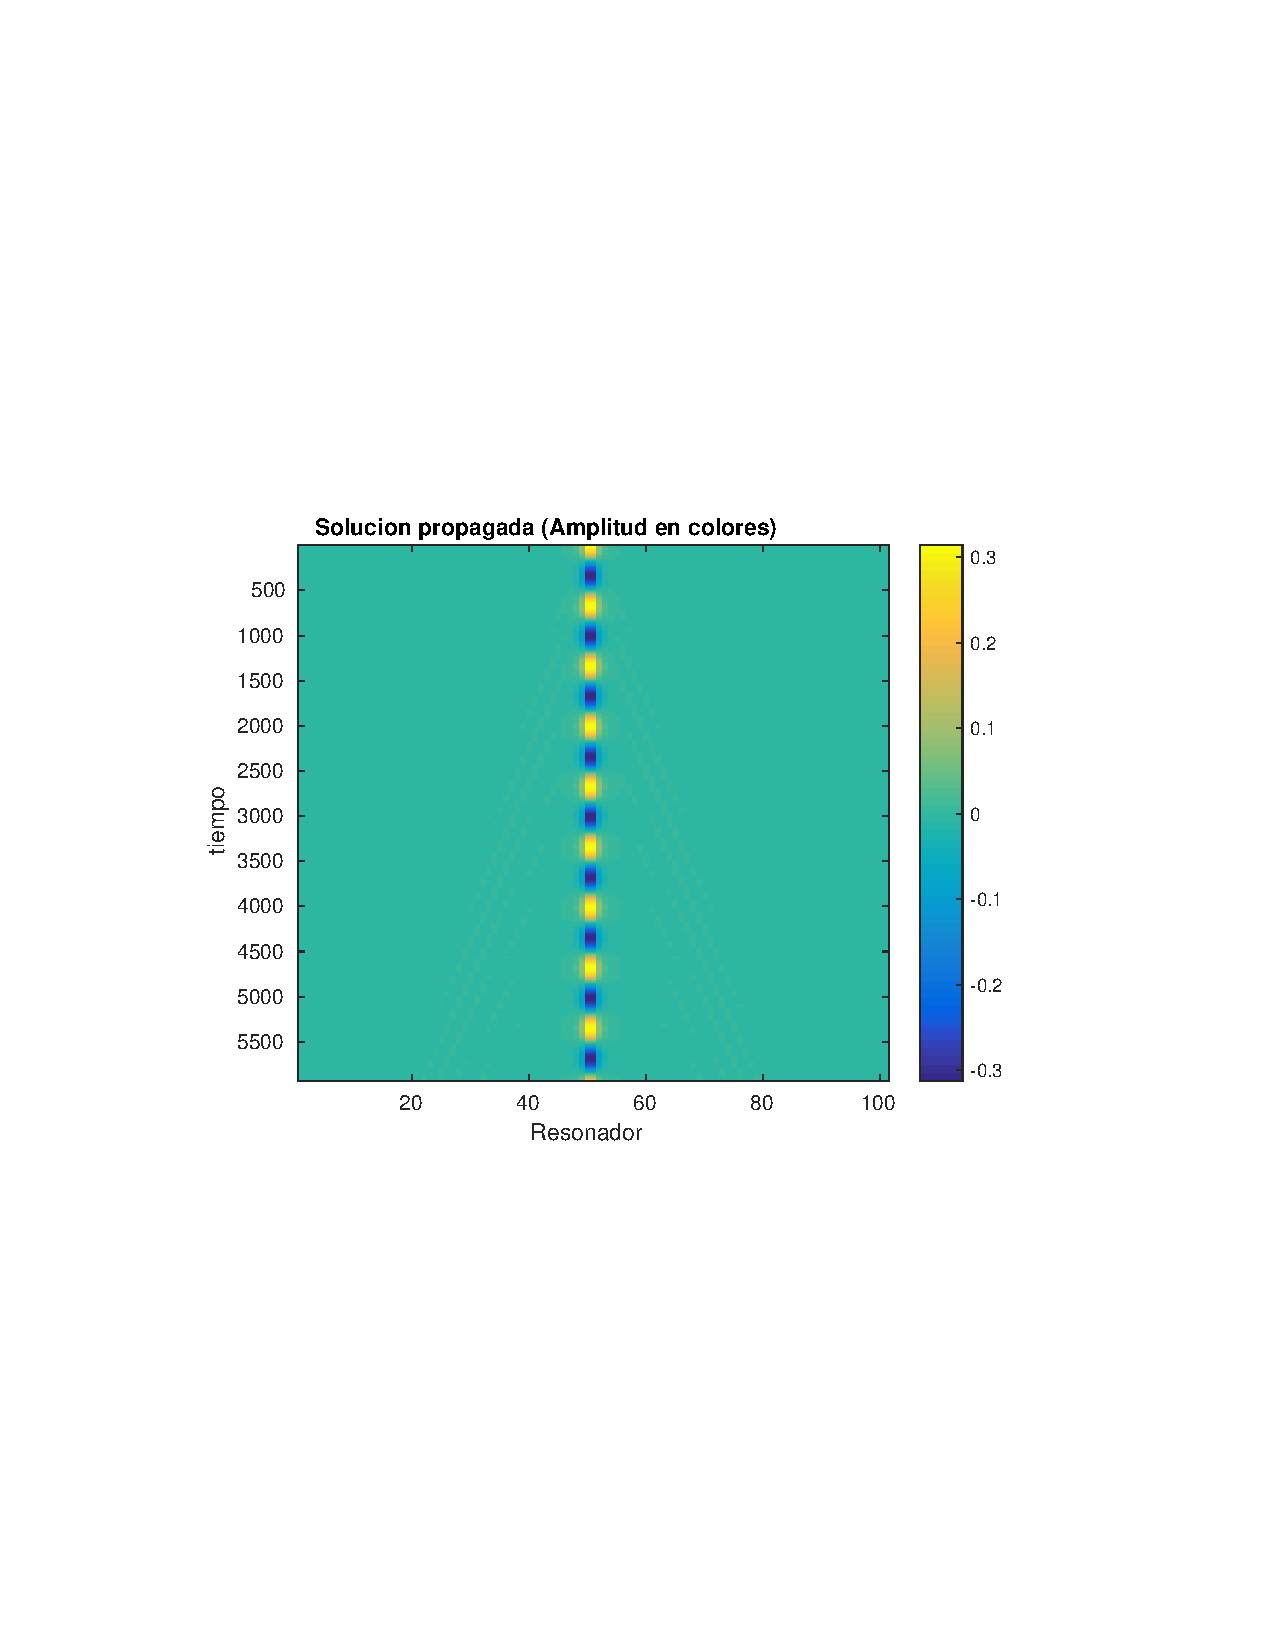
\includegraphics[scale=0.8]{SP2-40.pdf}
\end{figure}


\end{document}